\documentclass[aps,prd,onecolumn,superscriptaddress,nofootinbib]{revtex4-2}

% — Packages —
\usepackage[utf8]{inputenc}
\usepackage[T1]{fontenc}
\usepackage{lmodern}
\usepackage{amsmath,amssymb,bm,mathtools,amsthm}
\usepackage{graphicx}
\usepackage{adjustbox}
\usepackage{xcolor}
\usepackage{microtype}
\usepackage{enumitem}
\usepackage{tikz}
\usepackage{booktabs}
\usepackage{siunitx}

% — Hyperref (load last among packages) + robust PDF bookmarks —
\usepackage[unicode,pdfencoding=auto,psdextra]{hyperref}
\usepackage{bookmark}
\hypersetup{
  colorlinks=true,
  linkcolor=blue,
  citecolor=blue,
  urlcolor=blue
}

\sisetup{detect-all}
\usetikzlibrary{arrows.meta,positioning,fit,calc,shapes.geometric,shapes.multipart,backgrounds}

% — Colors for flowchart —
\definecolor{flowBlue}{HTML}{1F77B4}
\definecolor{flowPurple}{HTML}{9467BD}
\definecolor{flowGreen}{HTML}{2CA02C}
\definecolor{flowOrange}{HTML}{FF7F0E}
\definecolor{flowRed}{HTML}{D62728}
\definecolor{flowGray}{HTML}{7F7F7F}

% — PDF string sanitization —
\pdfstringdefDisableCommands{%
  \def\OmL{OmegaLambda}%
  \def\Omm{Omega m0}%
  \def\cgeo{cgeo}%
  \def\alphaM{alphaM}%
  \def\eps{epsilon}%
  \def\boxed#1{#1}%
  \def\mu{mu}%
  \def\alpha{alpha}%
  \def\alpha_M{alphaM}%
  \def\Omega_\Lambda{OmegaLambda}%
  \def\Gfield{Gfield}%
  \def\Sent{Sent}%
}

% — Math tweaks —
\allowdisplaybreaks

% — Macros —
\providecommand{\mpl}{M_{\rm P}}
\providecommand{\OmL}{\Omega_\Lambda}
\providecommand{\Omm}{\Omega_{m0}}
\providecommand{\cgeo}{c_{\rm geo}}
\providecommand{\alphaM}{\alpha_M}
\providecommand{\eps}{\varepsilon}
\providecommand{\be}{\begin{equation}}
\providecommand{\ee}{\end{equation}}
\providecommand{\bse}{\begin{subequations}}
\providecommand{\ese}{\end{subequations}}
\newcommand{\Gfield}{\mathcal{G}}
\newcommand{\Snt}{S_{\rm ent}}
\newcommand{\zenododoi}{10.5281/zenodo.TBD} % <– replace with final DOI before submission

% — Theorem-like environments —
\newtheorem{definition}{Definition}
\newtheorem{hypothesis}{Hypothesis}
\newtheorem{lemma}{Lemma}
\newtheorem{proposition}{Proposition}
\newtheorem{theorem}{Theorem}
\newtheorem{corollary}{Corollary}

\begin{document}

\title{Modular Response in Free Quantum Fields:\\
A KMS/FDT Theorem and Conditional Extensions}

\author{[clg]}
\affiliation{[Institutions]}
\date{}

\begin{abstract}
\textbf{Part I (Theoremic core, free/Gaussian Hadamard QFT).} We prove that, for small causal diamonds (CHM) in locally Hadamard states and within a safe window \(\epsilon_{\rm UV}\ll\ell\ll \min\{L_{\rm curv},\lambda_{\rm mfp},m_i^{-1}\}\), the MI/moment-kill projector isolates a finite \(\ell^4\) modular response with coefficient equal to its flat-space value; the projected KMS/FDT susceptibility is positive; and coarse-graining over the wedge family produces the universal weak-field prefactor \(5/12=(4/3)\times(5/16)\). The fractional KMS defect between CHM diamonds and half-spaces scales as \(\mathcal O((\ell/L_{\rm curv})^2)+\mathcal O((\ell H)^2)\). The QFT sensitivity is \(\beta=2\pi C_T I_{00}=0.02086\pm 0.00105\) (conservative \(5\%\) shared systematics). A scheme-invariant background relation \emph{suggests} \(\OmL=\beta\, f\,\cgeo\) \emph{conditional} on our coarse-graining and analyticity assumptions.

\smallskip
\textbf{Part II (Conditional extensions).} We separate \emph{definition} (flat-space \(\eps\) from modular response) from \emph{mapping}. Rather than impose the standard EFT-of-DE \(\alpha\)-basis, we adopt a quasi-static closure that keeps operational distances GR-like (no additional lensing coupling \(\Sigma\simeq 1\)) while modifying growth via \(\mu(\eps,s)=1/(1+\tfrac{5}{12}\eps\,s(x))\) with \(s(x)\) a local, covariant environment modulation derived from the action. KMS/FDT positivity motivates an entropy-driven law \(d\eps/d\ln a\ge 0\) with a \emph{conditional} background budget \(\int \eps\,d \ln a=\OmL\). We then prove a \emph{No-Go Lemma} showing any linear kernel fails to yield Tully–Fisher scaling and introduce a \emph{quasistatic elastic sector} (AQUAL form, derived as the SK static limit) with the \emph{same} fixed acceleration \(a_0=\frac{5}{12}\OmL^2 c H_0\). The elastic sector is convex, well-posed, obeys Solar–System curvature gating, produces \(\Phi=\Psi\) at working order (no slip), and leaves linear cosmology intact via a causal SK filter.

\smallskip
\textbf{Part III (Exploratory).} (i) An \emph{optional}, shock-selective \emph{optical} channel (D\(^{\prime}\)) reduces \(\Sigma\) only in high-shear shocked gas to address Bullet-type lensing offsets while preserving FRW distances, with a principled SK/BRSSS derivation path connecting the amplitude to ICM transport coefficients. (ii) A compact thermodynamic interpretation of the projected modular response: a Clausius-like identity holds at working order in the MI/moment-kill channel, and the FRW budget may be viewed as a \emph{coarse-grained} Clausius normalization \emph{conditional} on our KMS\(\to\)FRW hypotheses. (iii) \emph{Linkage to global entropic gravity (Bianconi 2025)} via small-diamond MI matching and observational discriminants.

\smallskip
\textbf{Referee-guided additions.} We (A) formalize an MI-smeared null-energy positivity (free fields; projected QEI), (B) make explicit the RG/operator-spectrum bridge pinning \(\beta\) to \(C_T\) and clarifying anomaly channels, (C) expose SM bookkeeping tied to the safe-window fraction \(f_V\) and curvature gating \(s(\chi_g)\) so that GR dominance is recovered wherever heavy sectors or strong curvature suppress the MI channel, and (D) add the \emph{No-Go Lemma + elastic SK/AQUAL sector} with fixed \(a_0\), no slip, Solar–System compliance, and cosmology/galaxy separation.
\end{abstract}

\maketitle

% ============================================================
\section*{Reader’s map: Part I (Theorem) vs.\ Part II (Conditional) vs.\ Part III (Exploratory)}
\noindent \textbf{Part I (Secs.~\ref{sec:scope}–\ref{sec:five-twelve}, \ref{sec:sm-link}, \ref{sec:referee-additions}A–B; Apps.~\ref{app:MI}–\ref{app:chm-kms-estimate}):} proven results for free/Gaussian Hadamard fields at working order, SM bookkeeping, and first-principles positivity/RG clarifications.\\
\textbf{Part II (Secs.~\ref{sec:def-vs-map}–\ref{sec:elastic}, \ref{sec:sk-separation}, \ref{sec:data}, \ref{sec:referee-additions}C; Apps.~\ref{app:fv}–\ref{app:microlocal}, \ref{app:entropic-proof}):} conditional mapping for growth (\(\mu(\eps,s)\)), \emph{Linear No-Go} (Sec.~\ref{sec:no-go}), and \emph{Elastic quasistatic sector} (Sec.~\ref{sec:elastic}) with Solar–System gating, no slip, and BTFR; causal SK separation of regimes.\\
\textbf{Part III (Secs.~\ref{sec:lemmaDprime}, \ref{sec:thermo}, \ref{sec:bianconi-link}; Apps.~\ref{app:SK}, \ref{app:SK-derivation}):} exploratory shock-selective optics (D\(^{\prime}\)); thermodynamic interpretation; and linkage to Bianconi’s global entropic gravity.

% ===============================
\section{Scope, Working Order, and Safe-Window Quantification (Part I)}
\label{sec:scope}

\paragraph{Working order and state class.} We work to \(\mathcal O(\ell^4)\) in the MI/moment-kill projector channel, treating curvature/contact terms as \(\mathcal O(\ell^6)\). States are locally Hadamard.

\paragraph{KMS applicability (CHM diamonds).} Exact BW KMS holds for half-spaces; CHM diamonds inherit it with fractional defect \(\mathcal O((\ell/L_{\rm curv})^2)+\mathcal O((\ell H)^2)\) (App.~\ref{app:chm-kms-estimate}).

\paragraph{Safe-window volume fraction.} Define a conservative admissible scale
\be
\label{eq:lmax}
\ell_{\max}(x)\equiv \zeta\,\min\Big\{L_{\rm curv}(x),\ \lambda_{\rm mfp}(x),\ m_i^{-1}(x)\Big\},\qquad \zeta=0.1.
\ee
Using Press–Schechter/Sheth–Tormen mass functions and NFW curvature proxies \(L_{\rm curv}^{-2}\sim (R_{abcd}R^{abcd})^{1/2}\) with substructure excision parameter \(\xi\), we estimate the comoving volume fraction \(f_V(\ell_{\min})=\mathrm{Vol}\{x:\,\ell_{\max}(x)>\ell_{\min}\}/\mathrm{Vol}_{\rm tot}\). A semi-analytic survey (App.~\ref{app:fv}) shows voids dominate \(f_V\), while dense cores lack a window; representative values at \(z\!\sim\!0\) for \(\ell_{\min}\in[1,100]\) pc are \(f_V\sim 0.6{-}0.95\) for \(\xi\in[0.2,0.5]\). This enters only as a domain-of-validity indicator.

\paragraph{Spectrum caveat.}
The admissible window \(\epsilon_{\rm UV}\ll \ell\ll\min\{L_{\rm curv},\lambda_{\rm mfp},m_i^{-1}\}\) is understood to apply to sectors that contribute at working order. Massive sectors with \(\ell\gg m_i^{-1}\) are exponentially suppressed and, after MI/moment–kill subtraction, do not re‑introduce lower moments or \(\ell^4\log\ell\) terms. Thus the \(\ell^4\) coefficient is dominated by massless/light fields while heavy fields decouple in this channel. \emph{See Sec.~\ref{sec:sm-link} for SM bookkeeping that packages light-field multiplicity into a single \(\varepsilon_{\rm SM}\).}

\paragraph{Angle invariance as a null test.} The continuous-angle product \(\mathcal C_\Omega=f(\theta)\,\cgeo(\theta)\) is analytic and \(\theta\)-independent; residuals are shown as a null check, not a precision claim.

% ===============================
\section{A2–KMS Theorem (Gaussian/Hadamard Sector)}
\label{sec:theorem}

\begin{theorem}[Projected modular response and positivity]\label{thm:proj-modresp}
Let \(\mathcal Q\) be a free (Gaussian) QFT on a globally hyperbolic spacetime and \(\rho\) a locally Hadamard state. For a causal diamond of radius \(\ell\) with \(\ell\ll L_{\rm curv}\) and the MI/moment-kill projector that cancels \(r^0\) and \(r^2\) moments, the MI-subtracted modular response obeys
\be
\delta\!\langle K_{\rm sub}\rangle=(2\pi C_T I_{00})\,\ell^4\,\delta\eps+\mathcal O(\ell^6),
\ee
with coefficient equal to the flat-space value. The retarded susceptibility \(\chi_{QK}\) in the projected channel is positive (FDT), and wedge averaging yields the universal weak-field prefactor \(5/12\). The fractional deviation from BW KMS is \(\mathcal O((\ell/L_{\rm curv})^2)+\mathcal O((\ell H)^2)\).
\end{theorem}

\begin{corollary}[Conditional background statement]\label{cor:background-cond}
Under the coarse-graining and analyticity assumptions of Sec.~\ref{sec:kms-frw}, the FRW zero mode \emph{suggests} the scheme-invariant relation
\(\OmL=\beta\,f\,\cgeo\) with \(\beta=2\pi C_T I_{00}\). We treat this as a conditional statement rather than a theorem.
\end{corollary}

% ===============================
\section{QFT Input: \texorpdfstring{$\beta=2\pi C_T I_{00}$}{beta} and Error Budget}
\label{sec:beta}
We evaluate \(\beta\) via four independent routes: (a) real-space CHM; (b) spectral/Bessel; (c) Euclidean time-slicing; (d) replica finite-difference. The spread is \(\lesssim 1\%\). We adopt a conservative
\be
\beta=0.02086\pm 0.00105 \quad (5\%~\text{shared systematics}).
\ee
Angle invariance is used as a null residual test.

\noindent Here \(C_T\) denotes the flat-space stress-tensor two-point normalization, e.g.
\(\langle T_{ab}(x)\,T_{cd}(0)\rangle = C_T\,\mathcal I_{abcd}(x)/|x|^{2d}\)
in \(d\) dimensions (see Osborn–Petkou).

\noindent\emph{Benchmark (convention).} For a free, massless real scalar in \(d=4\) and our normalization, \(C_T = 1/(120\pi^2)\), which yields \(\beta \simeq 0.02086\) via Eq.~\eqref{eq:eps-def}.

\noindent\textbf{Implementation consistency (note).} The normative constants used for the numerical reproductions are
\[
C_T=\frac{1}{120\pi^2},\qquad (\sigma_1,\sigma_2)=\Big(\tfrac{1}{2},2\Big),\qquad (a,b)=\Big(\tfrac{4}{5},\tfrac{1}{5}\Big),
\]
with the moment-kill identities enforced exactly (App.~\ref{app:MI}). Helper scripts (\texttt{beta\_methods\_v2.py}, \texttt{referee\_pipeline.py}) print these values alongside the computed \(I_{00}\) to prevent normalization drift.\footnote{In earlier development branches some convenience flags defaulted to alternate normalizations (e.g.\ \(C_T=3/\pi^4\)) and near-unity MI scales. These have been disabled in the archival runners; the paper’s conventions are authoritative.}

\noindent\textbf{Reproducibility (non‑circular).} We use a two–scale MI/moment‑kill subtraction with a top‑hat window on 3‑balls
\[
W_\ell(r)=\frac{3}{4\pi \ell^3}\,\Theta(\ell-r),\qquad
\mathcal{W}_\ell:=\int_{B_\ell}\!W_\ell-\;a\!\int_{B_{\sigma_1\ell}}\!W_{\sigma_1\ell}-\;b\!\int_{B_{\sigma_2\ell}}\!W_{\sigma_2\ell}.
\]
The two moment‑kill conditions (cancelling \(r^0\) and \(r^2\) for any smooth radial \(F\)) fix
\[
a+b=1,\qquad a\,\sigma_1^2+b\,\sigma_2^2=1
\ \ \Longrightarrow\ \
a=\frac{\sigma_2^2-1}{\sigma_2^2-\sigma_1^2},\quad
b=\frac{1-\sigma_1^2}{\sigma_2^2-\sigma_1^2}.
\]
In our runs we take
\[
(\sigma_1,\sigma_2)=\Big(\tfrac{1}{2},\,2\Big),\qquad (a,b)=\Big(\tfrac{4}{5},\,\tfrac{1}{5}\Big)=(0.8,0.2).
\]
With these weights the projected \(\ell^4\) coefficient evaluates to
\[
I_{00}=3.932017\ \ \text{(dimensionless)},
\]
so with \(C_T=1/(120\pi^2)\) one obtains \(\beta=2\pi C_T I_{00}=0.02086\) as quoted. The helper script \texttt{beta\_methods\_v2.py} echoes both \((a,b;\sigma_1,\sigma_2)\) and the numeric \(I_{00}\).

% ===============================
\section{Standard-Model sector: bookkeeping and decoupling at working order}
\label{sec:sm-link}

\paragraph{What is being linked.}
At working order the MI/moment–kill channel defines the dimensionless state variable \(\varepsilon(x)\) through
\[
\delta\!\langle K_{\rm sub}\rangle=\beta\,\ell^4\,\delta\varepsilon+\mathcal O(\ell^6)
\quad\text{[Eq.~\eqref{eq:eps-def}].}
\]
This subsection clarifies how the \emph{Standard–Model (SM)} content enters \(\varepsilon\) and why heavy states decouple.

\paragraph{Species sum and decoupling.}
Write \(\varepsilon\) as a weighted sum over species \(i\):
\[
\varepsilon(x)=\sum_{i}w_i\,\varepsilon_i(x),\qquad
w_i\ \text{counts effective dof (helicity/polarization, internal factors)}.
\]
In a diamond of size \(\ell\), fields with \(m_i\ell\gg 1\) are exponentially suppressed in the projected channel; after the MI/moment–kill subtraction they do \emph{not} re‑introduce lower moments nor \(\ell^4\log\ell\) terms. Parametrically,
\[
\varepsilon_i(x)\ \propto\ e^{-m_i\ell}\quad\text{for }m_i\ell\gg 1,
\]
so the \(\ell^4\) coefficient is dominated by massless/light fields while heavy fields decouple.

\paragraph{Packaging the light SM content.}
It is convenient to define a single light‑sector variable
\[
\varepsilon_{\rm SM}(x)\equiv\sum_{i\in \text{light}} c_i\,\varepsilon_i(x),
\]
where \(c_i\) packages the relevant multiplicities (helicity/polarization, internal quantum numbers) of each light SM species under the MI projection. All subsequent working‑order formulas may then be read with \(\varepsilon\to \varepsilon_{\rm SM}\) when SM content is explicitly considered.

\paragraph{Coupling to gravity at working order.}
The only background scalar that survives the MI/moment–kill projection and modifies weak‑field growth while keeping distances GR‑like is the Planck‑mass renormalization \(\delta\!\ln M^2=\beta\,\delta\varepsilon\) (Assumption~D). Multiplicities therefore simply rescale \(\varepsilon\) (hence \(\mu\)); they do \emph{not} change \(\beta\) or the universal weak‑field bookkeeping that fixes the \(5/12\) prefactor:
\[
\mu(\varepsilon,s)=\frac{1}{1+\tfrac{5}{12}\,\varepsilon\,s(x)}
\quad\longrightarrow\quad
\mu(\varepsilon_{\rm SM},s)=\frac{1}{1+\tfrac{5}{12}\,\varepsilon_{\rm SM}\,s(x)}.
\]

\paragraph{Environment and distances.}
The environment scalar \(s(x)\) is geometric (built from curvature invariants) and independent of particle content at this order; FRW distances remain GR‑like (\(\Sigma\simeq 1, c_T=1\)). The observed lensing amplitude changes only indirectly through altered growth.

\paragraph{Practical note and $f_V$ linkage.}
In cosmological applications one sets a light‑sector threshold \(m_i\ell\lesssim 1\) (with \(\ell\) within the safe window) and computes \(\varepsilon_{\rm SM}\) using the appropriate \(c_i\). As the environment varies, \emph{field regimes can re‑enter} \(\varepsilon_{\rm SM}\) smoothly. Dense regions with no safe window contribute negligibly to the MI channel; voids dominate the valid domain via \(f_V\) (App.~\ref{app:fv}). GR dominance is ensured either by strong curvature (\(s(\chi_g)\!\to\!0\)) or by heavy-sector decoupling (\(m_i\ell\!\gg\!1\)).

% ===============================
% ===============================
\section{Weak-Field Prefactor \texorpdfstring{$5/12$}{5/12}}
\label{sec:five-twelve}
The isotropic BW channel gives \(\langle T_{kk}\rangle=(1+w)\rho\) with UV \(w=1/3\Rightarrow 4/3\).
Averaging over CHM segments yields \(5/16\), so \(5/12=(4/3)\times(5/16)\).
Details in Sec.~\ref{sec:five-twelve}.

% ============================================================
\section{Definition vs.\ Mapping (Part II; Conditional)}
\label{sec:def-vs-map}

\paragraph{Definition (flat-space QFT).}
\be
\label{eq:eps-def}
\delta\!\langle K_{\rm sub}(\ell)\rangle=\underbrace{(2\pi C_T I_{00})}_{\beta}\,\ell^4\,\delta\eps(x)+\mathcal O(\ell^6).
\ee

\paragraph{Mapping (constitutive; beyond the \texorpdfstring{$\alpha$}{alpha}-basis).}
We \emph{do not} impose the linear EFT-of-DE \(\alpha\)-parameter mapping at working order. Instead, we adopt a quasi-static closure that keeps operational distances GR-like while modifying growth:
\bse
\label{eq:qs-closure}
\be
\nabla^2\Phi \;=\; 4\pi G a^2 \rho_m \,\mu(\eps,s), \qquad
\mu(\eps,s)=\frac{1}{1+\tfrac{5}{12}\eps\,s(x)},
\ee
\be
\nabla^2\frac{\Phi+\Psi}{2} \;=\; 4\pi G a^2 \rho_m ,\qquad (\Sigma\simeq 1\ \text{on FRW and in laminar flows}).
\ee
\ese
Here \(s(x)\) is a local scalar built from curvature (Sec.~\ref{sec:env}); in FRW, Weyl \(=0\Rightarrow \chi_g=0\Rightarrow s=1\).
\emph{Beyond working order we make no stability claims absent an action; \(\mu(\varepsilon,s)\) serves as a falsifiable diagnostic with \(\Sigma\simeq 1\).}
Matter obeys the standard continuity and Euler equations. This closure preserves the Bianchi identity at working order because \(s(x)\) is a scalar; an action-level realization and frame‑independence are given below (Remark~\ref{sec:throttle-remark}). \emph{Optional Assumption D\(^{\prime}\) (Sec.~\ref{sec:lemmaDprime})} introduces a \emph{shock-selective} lensing modification \(\Sigma(x)<1\) localized to high-shear gas while keeping FRW \(\Sigma\simeq 1\).

\noindent\emph{Remark on lensing amplitude.} \(\Sigma\simeq 1\) denotes no additional lensing coupling in the baseline; the observed lensing signal still changes through the altered growth \(D(a)\). Under Assumption~D\(^{\prime}\), \(\Sigma\) may be reduced \emph{locally} in shocked gas (\(\mathcal S_{\rm shock}\gg 1\)) without affecting FRW.

\paragraph{EFT stub (derivation of \(5/12\)).}
At quasi-static, sub-horizon scales, a background variation \(\delta\ln M^2=\beta\,\delta\varepsilon\) rescales the Poisson coupling as \(G\!\to\!G_{\rm eff}=G/(1+\Delta)\) with \(\Delta\) fixed by the universal weak-field bookkeeping. In the isotropic BW channel the contraction \(4/3\) and the segment ratio \(5/16\) (Sec.~\ref{sec:five-twelve}) give \(\Delta=\tfrac{5}{12}\varepsilon\), hence
\be
\mu(\varepsilon,s)=\frac{G_{\rm eff}}{G}=\frac{1}{1+\tfrac{5}{12}\varepsilon\,s(x)},
\label{eq:eft-stub}
\ee
consistent with Eqs.~\eqref{eq:qs-closure}.

\paragraph{Trial action (outlook).}
A possible action-level route consistent with our closure is to consider an effective term that modulates \(M^2\) via the modular response,
\[
S_{\rm trial}=\int d^4x \,\sqrt{-g}\left[\frac{M^2}{2}R + \lambda\,(\delta\!\ln M^2)\,\mathcal{K}[g;\ell] + \cdots\right],
\]
where \(\mathcal K\) is a local covariant scalar capturing the projected channel at working order and \(\lambda\) a running coefficient. While only illustrative, this shows how \(\delta\!\ln M^2=\beta\,\delta\varepsilon\) could arise from an action (cf.\ \cite{Jacobson2016,Lashkari2014}).

\subsection{Frame-independence of throttling (remark)}
\label{sec:throttle-remark}
\emph{Throttling} here means the reduction of the effective gravitational coupling relative to GR caused by the background state variable \(\varepsilon(a)\) and a local environment factor \(s(x)\) that encodes curvature/inhomogeneity.
In the Jordan frame we take
\[
M_*^2(x,a)=M^2\!\left[1+\tfrac{5}{12}\,\varepsilon(a)\,s(x)\right],\qquad
s(x)=\frac{1}{1+(\chi_g/\chi_\star)^q}+\mathcal O\!\Big(\frac{R}{m_s^2}\Big),
\]
so the quasi-static Poisson law reads
\[
\nabla^2\Phi \simeq \frac{4\pi G a^2 \rho_m\,\delta}{1+\tfrac{5}{12}\,\varepsilon(a)\,s(x)}
\quad\Rightarrow\quad
G_{\rm eff}(x,a)=\frac{G}{1+\tfrac{5}{12}\,\varepsilon(a)\,s(x)}.
\]
Thus throttling is present everywhere, while its magnitude is amplitude–modulated by the local invariant \(\chi_g=\ell^2\sqrt{C_{abcd}C^{abcd}}\): in weak fields (\(\chi_g\!\ll\!\chi_\star\)) one has \(s\!\to\!1\) and the full background rescaling \(G_{\rm eff}=G/(1+\tfrac{5}{12}\varepsilon)\); in strong fields (\(\chi_g\!\gg\!\chi_\star\)) one has \(s\!\to\!0\) and \(G_{\rm eff}\!\to\!G\) (Solar–System compliance).

A conformal map to the Einstein frame,
\[
\tilde g_{\mu\nu}=\Omega^2 g_{\mu\nu},\qquad \Omega^2=1+\tfrac{5}{12}\,\varepsilon(a)\,s(x),
\]
renders \(M_*\) constant and shifts the same throttling into the matter coupling. To working order in our MI/moment-kill channel, gradients of \(\Omega\) and of \(\chi_g\) enter only at \(\mathcal O\!\big((\ell/L_{\rm curv})^2\big)\) and \(\mathcal O(R/m_s^2)\), consistent with the error budget in Eq.~\eqref{eq:chi-defect} and App.~\ref{app:chm-kms-estimate}; the observables of interest are frame–independent at this order: growth is governed by
\[
\mu(\varepsilon,s)=\frac{1}{1+\tfrac{5}{12}\,\varepsilon(a)\,s(x)},
\]
and distances remain GR-like (\(\Sigma\simeq 1\), \(c_T=1\)).\footnote{This remark complements Assumption~D (Sec.~\ref{sec:lemmaD}): the working-order modification resides in a state- and environment-dependent \(M_*^2\) with no additional lensing coupling. A failure would manifest as our falsifiers in Sec.~\ref{sec:program}, e.g.\ a significant GW/EM distance split or a persistent \(\ell^4\log\ell\) term.}

\noindent\emph{Scale-separation note.} The \emph{local} modular response enters gravity solely as a renormalization \(\delta\!\ln M_*^2=\beta\,\delta\varepsilon\) of the Planck mass; the Einstein equations then propagate this renormalization to cosmological scales through the standard gravitational coupling. No macroscopic quantum coherence or ad hoc coarse-graining is required, and the Jordan\(\leftrightarrow\)Einstein map above makes this statement frame-independent at working order.

A simple way to realize \(s(x)\) is as an auxiliary heavy scalar that minimizes a local potential
\[
\mathcal V(s;\chi_g)=\frac{M^2 m_s^2}{2}\left[s-\frac{1}{1+(\chi_g/\chi_\star)^q}\right]^2,
\]
so that the algebraic EOM enforces \(s=[1+(\chi_g/\chi_\star)^q]^{-1}+\mathcal O(R/m_s^2)\). Choosing \(m_s^2\!\gg\!H_0^2\) ensures adiabatic tracking.

\noindent\textbf{Constraints (working order).}
(i) Choose \(m_s^2\gg H_0^2\) so \(s(x)\) adiabatically tracks \([1+(\chi_g/\chi_\star)^q]^{-1}\) and the \(\mathcal O(R/m_s^2)\) offset is negligible.
(ii) The Planck-mass drift \(\alpha_M=d\ln M_*^2/d\ln a=\frac{(5/12)\,s\,d\varepsilon/d\ln a}{1+(5/12)\varepsilon s}\) is naturally small under our monotone \(\varepsilon(a)\).
(iii) In FRW, Weyl \(=0\) so curvature-weighted corrections vanish; in LSS they are \(\mathcal O\!\big((\ell/L_{\rm curv})^2\big)\).

\noindent \emph{Weak-field acceleration (toy/conditional; clarification).} Because \(s\!\to\!1\) in low curvature, the weak-field normalization implies a MOND-like scale
\be
a_0=\frac{5}{12}\,\OmL^2\,c\,H_0,
\ee
Using the baseline \(\OmL=0.685\) and \(H_0=70.9~\mathrm{km\,s^{-1}\,Mpc^{-1}}\), this gives \(a_0^{\rm eff}\approx 1.2\times 10^{-10}\,\mathrm{m\,s^{-2}}\) in the weak-field limit (\(s\simeq 1\));
and the effective \(a_0^{\rm eff}\) is \emph{enhanced} in weak-field regimes by the \emph{derived} \(s\!\to\!1\) (not imposed), while Solar–System compliance follows from \(s(\chi_\odot)\ll 1\) (Sec.~\ref{sec:env}). Pipeline values propagate the \(\pm 5\%\) uncertainty in \(\beta\).

% ===============================
\section{Linear-kernel No-Go for Tully–Fisher}
\label{sec:no-go}

\begin{lemma}[Linear-kernel no-go]\label{lem:nogo}
Let \(\Phi\) be determined from \(\rho\) by a translation/rotation-invariant \emph{linear} map with tempered kernel \(G\):
\[
\Phi(\mathbf{x})=(G * \rho)(\mathbf{x}),\qquad  
G(\mathbf{x})=\frac{1}{(2\pi)^3}\!\int \frac{\tilde g(\mathbf{k})}{k^2}\,e^{i\mathbf{k}\cdot\mathbf{x}}\,d^3k,\ \ \tilde g(\mathbf{k})>0,
\]
and assume that outside a bounded mass distribution the stationary field equation reduces to a linear constant-coefficient elliptic operator. Then the exterior field decays as \(\Phi\sim -\mathcal G_{\rm eff} M/r\), so \(g=|\nabla\Phi|=\mathcal G_{\rm eff}GM/r^2+o(r^{-2})\) and \(v_\infty^4\propto M^2\). Thus a linear kernel \emph{cannot} yield the Tully–Fisher scaling \(v_\infty^4\propto M\).
\end{lemma}

\noindent\emph{Sketch.} In vacuum the solution is harmonic (up to renormalization \(\mathcal G_{\rm eff}\)); Liouville/Rellich imply the only decaying solution is \(1/r\), hence \(g\propto r^{-2}\). Any linear, isotropic nonlocality rescales \(\mathcal G_{\rm eff}\) but preserves the \(1/r^2\) falloff.

% ===============================
\section{Elastic quasistatic sector (AQUAL from SK static limit)}
\label{sec:elastic}

\paragraph{Static elastic action and field equation.}
In the quasistatic limit of the Schwinger–Keldysh (in–in) effective action, a causal retarded kernel \(\mathcal K^{\rm el}\) reduces to a local, convex functional for the Newtonian potential \(\Phi\):
\[
\boxed{\ \mathcal L_{\rm el}(\Phi,\nabla\Phi) \;=\; \frac{a_0^2}{8\pi G}\,F\!\left(Y\right)\;-\;\rho\,\Phi,\quad Y\equiv \frac{|\nabla\Phi|^2}{a_0^2}\ }
\]
with \(F\in C^2([0,\infty))\), \(F'(Y)=\mu(Y)>0\), \(F''(Y)\ge0\), and asymptotics
\[
\mu(Y)\xrightarrow{Y\gg1} 1,\qquad \mu(Y)\xrightarrow{Y\ll1} \sqrt{Y}.
\]
Variation yields the AQUAL field equation \cite{BekensteinMilgrom1984}:
\be
\nabla\!\cdot\!\big(\mu(Y)\,\nabla\Phi\big)=4\pi G\,\rho.
\ee

\paragraph{Deep regime and BTFR (galaxies).}
For spherical mass \(M\), in the deep regime (\(g\ll a_0\Rightarrow \mu\simeq\sqrt{Y}=g/a_0\)) one obtains
\[
\frac{g}{a_0}\,g=\frac{GM}{r^2}\quad\Rightarrow\quad g(r)=\frac{\sqrt{GMa_0}}{r},\qquad v_\infty^4=GMa_0.
\]
Thus the baryonic Tully–Fisher relation follows directly.

\paragraph{Uniform ellipticity / well-posedness.}
The linearization tensor
\[
\mathcal A_{ij}(\nabla\Phi)=\mu\,\delta_{ij}+\frac{2\mu'}{a_0^2}\,\partial_i\Phi\,\partial_j\Phi
\]
is uniformly elliptic provided \(\mu>0\) and \(\mu+2Y\mu'(Y)>0\), which holds for the convex class above. Existence/uniqueness follows from standard elliptic theory.

\paragraph{Canonical convex interpolant (parameter-free).}
A simple, convex, parameter-free choice with the required asymptotics is
\[
\boxed{\ \mu(Y)=\frac{\sqrt{Y}}{1+\sqrt{Y}}\ },\qquad
F(Y)=\int_0^Y \mu(s)\,ds=Y-2\sqrt{Y}+2\ln(1+\sqrt{Y}).
\]
No dimensional parameter beyond \(a_0\) is introduced.

\paragraph{Same fixed acceleration scale.}
We identify
\[
\boxed{\ a_0=\frac{5}{12}\,\Omega_\Lambda^2\,c\,H_0\ }
\]
from the capacity (Part~I/II) channel; thus the BTFR normalization is **fixed** (no fit).

\paragraph{Solar–System compliance (curvature gate).}
Insert the same curvature gate via \(a_0\!\to\! a_0^{\rm eff}(x)=a_0\,s(\chi_g)^p\) (with \(p\ge1\) integer). Using Sec.~\ref{sec:env} one has \(s(\chi_\odot)\lesssim 10^{-5}\), hence \(a_0^{\rm eff}\ll 10^{-15}\,a_0\) in the Solar System, fully suppressing elastic effects.

\paragraph{Lensing equals dynamics (no slip).}
Place the static elastic density in the quasistatic Einstein system symmetrically so that \(\Phi=\Psi\) at working order; equivalently, couple the AQUAL density to \((\Phi+\Psi)/2\). Then the lensing potential \(2\Phi\) tracks the same \(\mu\) that governs dynamics, and galaxy–galaxy lensing matches rotation-curve inferences.

% ===============================
\section{Causal SK separation of cosmology vs.\ galaxies}
\label{sec:sk-separation}
In the full SK theory, the elastic kernel depends on frequency and wavenumber, \(\mathcal K^{\rm el}(\omega,k)\). Causality and finite relaxation imply a factor
\[
\mathcal K^{\rm el}(\omega,k)=\mathcal Q(\omega,k)\,\mathcal K^{\rm el}(0,k),\qquad \mathcal Q(0,k)=1,\ \ |\mathcal Q(\omega\sim H,k\lesssim k_{\rm LSS})|\ll 1.
\]
Thus:
\begin{itemize}[leftmargin=*,noitemsep,topsep=0pt]
\item \textbf{Linear cosmology (FRW, LSS):} \(\omega\!\sim\!H,\,k\!\lesssim\!k_{\rm LSS}\Rightarrow \mathcal Q\!\approx\!0\). Dynamics is governed by the \emph{capacity channel} (\(\mu(\eps,s)<1\)), preserving distances and the \(S_8\) suppression.
\item \textbf{Quasistatic galaxies:} \(\omega\!\to\!0,\,k\!\gtrsim\!k_{\rm gal}\Rightarrow \mathcal Q\!\to\!1\). The \emph{elastic} AQUAL sector governs dynamics and lensing with fixed \(a_0\).
\end{itemize}
No new dimensional scales are introduced; \(\mathcal Q\) encodes scale separation already present in the SK influence functional.

% ===============================
\section{Covariant KMS \texorpdfstring{$\to$}{->} FRW Link and Error Control}
\label{sec:kms-frw}
Let \(s\) denote modular time with \(\beta_{\rm KMS}=2\pi/\kappa\) locally, where \(\kappa\) is the local boost surface gravity so that the approximate conformal Killing field \(\xi^a\) satisfies \(\xi^a\nabla_a=\kappa\,\partial_s\).
Averaging the retarded kernel over a comoving congruence of diamonds and reparametrizing \(s\mapsto \ln a\) induces the FRW background factor \(f\,\cgeo\); diffeomorphism covariance is preserved because the averaging functional depends only on local curvature scalars and the diamond foliation. The total fractional defect in the kernel obeys
\be
\label{eq:chi-defect}
\frac{\delta\chi}{\chi_{\rm BW}}=\mathcal O\!\Big((\ell/L_{\rm curv})^2\Big)+\mathcal O\!\big((\ell H)^2\big)
\ \ \approx\ \ 10^{-12}+10^{-18}
\ee
for \(\ell\!\sim\!10\,\mathrm{pc}\), \(L_{\rm curv}\!\sim\!10\,\mathrm{Mpc}\), \(H^{-1}\!\sim\!4\,\mathrm{Gpc}\).

\begin{proposition}[FRW budget identity (conditional; analyticity hypothesis)]
\label{prop:frw-budget}
Assume: (H1) locality and rapid decay of the spatially averaged, projected retarded kernel so that its reparametrization defines a distribution in \(\ln a\); (H2) adiabatic evolution through matter domination so that \(J(a)=ds/d\ln a\propto H(a)^{-1}\) varies slowly; (H3) preservation of KMS analyticity of the averaged kernel under the reparametrization \(s\!\to\!\ln a\); and (H4) negligible CHM vs.\ half-space deviation at working order (App.~\ref{app:chm-kms-estimate}). Then
\[
\Big\langle \!\int \chi^{\rm proj}_{QK}(a,a')\,d^3x \Big\rangle
= \beta\, f\, \cgeo\, \delta(\ln a-\ln a') + \ldots
\]
and integrating the entropy-driven evolution \(d\eps/d\ln a=\sigma(a)I(a)\ge0\) yields the coarse-grained identity
\be
\int_{a_i}^{1}\!\eps(a)\,d\ln a \;=\; \OmL \;=\; \beta\, f\,\cgeo,
\label{eq:budget}
\ee
used as a normalization under (H1)–(H4).
\end{proposition}
\noindent\emph{Operational diagnostic.} The routine \texttt{referee\_pipeline.py} reports a scalar residual \(R_{\rm nonloc}\equiv\sum_{i\neq 0}\big|\bar\chi^{\rm proj}(\Delta_i)\big|\,\Delta(\ln a)_i\) outside the contact bin; by default we take the central bin(s) with \(|\Delta(\ln a)|\le \Delta_0\) as ``contact''. Declare failure if \(R_{\rm nonloc}/\sigma_{\rm boot}>3\) \emph{and} the contact weight \(w_0<0.95\).

\paragraph{Rigor note.}
A full microlocal proof of (H3)—preservation of KMS analyticity under the coarse-grained reparametrization \(s\!\to\!\ln a\)—is deferred to future work in the spirit of Hollands–Wald~\cite{HollandsWald2001}.

\paragraph{Thermodynamic analogy (pointer).}
The entanglement first law suggests a Clausius-like analogy (Sec.~\ref{sec:thermo}), \emph{conditional} on (H1)–(H4), with MI projection avoiding CGM’s marginality issues (App.~\ref{app:microlocal}).

% ===============================
\section{Referee-guided first-principles closures and tests}
\label{sec:referee-additions}

\subsection*{A. MI-smeared null-energy bound (projected; proven for free fields)}
\noindent\textbf{Statement (free/Gaussian sector).} Let \(k^a\) be a null generator of the CHM diamond and \(h_\ell(x)\ge0\) a smooth, compactly supported sampling function adapted to the MI window (normalized to unit weight). Define the MI-smeared null contraction
\[
\mathcal{E}^{\rm MI}_\ell \;\equiv\; \int\! d^4x\,d^4x'\,h_\ell(x)\,h_\ell(x')\, \langle T_{ab}(x)k^a k^b \rangle_{\rm sub}^{\rm proj}\;.
\]
Then, in free Hadamard theories,
\[
\mathcal{E}^{\rm MI}_\ell \;=\; \underbrace{\langle \delta K_{\rm sub},\,\delta K_{\rm sub}\rangle_{\rm BKM}}_{\ge 0}\;\times\; \mathcal{N}_\ell
\quad\Rightarrow\quad
\mathcal{E}^{\rm MI}_\ell \ge 0
\]
with a calculable \(\ell\)-dependent normalization \(\mathcal N_\ell>0\) fixed by the MI projector.

\smallskip
\noindent\emph{Consequence.} The MI/moment-kill subtraction yields a \emph{QEI-like} positive quadratic form for null energy in the projected channel (free fields: exact; interacting: Assumption C).

\subsection*{B. RG/operator-spectrum bridge and anomaly guardrails}
\noindent\textbf{Bridge.} \(\beta\) is tied to the stress-tensor two-point normalization \(C_T\); our \(\ell^4\) universality relies on the MI projector removing \(\Delta<4\) contributions. Protected marginal operators would show up as \(\ell^4\log\ell\) in this channel; the \emph{absence} of such a term (checked numerically) is therefore a guardrail (Sec.~\ref{sec:program}, (i)).

\noindent\textbf{Anomalies.} Parity-odd and trace-anomaly structures do not contribute at \(\mathcal O(\ell^4)\) in the MI-projected, parity-even channel; they either vanish by symmetry or are curvature-suppressed by \(\mathcal O((\ell/L_{\rm curv})^2)\).

\subsection*{C. Where GR dominates: $f_V$ \& curvature gating (SM-aware)}
\noindent Dense, high-curvature regions either (i) lack a safe window (small \(f_V\) locally) or (ii) trigger \(s(\chi_g)\to 0\) so that \(G_{\rm eff}\to G\). Heavy SM sectors drop out when \(m_i\ell\gg 1\). Thus GR dominance is guaranteed wherever MI control fails or curvature is large, while voids (dominant in \(f_V\)) carry the clean MI signal.

% ===============================
\section{Assumptions for Interacting Extensions at Working Order (Part II; stated and test criteria)}
\label{sec:proofs}

\subsection{Assumption C (stated; test criteria): Relative entropy \texorpdfstring{$\leftrightarrow$}{<->} canonical energy in the projected diamond}
\label{sec:lemmaC}
\noindent\textbf{Statement.} For a local algebra \(\mathcal A(B_\ell)\) of an interacting Hadamard QFT obeying the microlocal spectrum condition and time-slice axiom, the MI/moment-kill projected second variation of Araki relative entropy equals the canonical-energy quadratic form of the projected stress tensor, up to \(\mathcal O(\ell^6)\) remainders, with a positive-definite projected kernel \(\chi_{QK}^{\rm proj}\).

\smallskip
\noindent\textbf{Rationale (sketch).} (i) The second variation is the Bogoliubov–Kubo–Mori metric. (ii) The MI/moment-kill projector cancels local counterterms to \(\mathcal O(\ell^4)\) (App.~\ref{app:MI}), conjectured to persist in interacting Hadamard QFTs (App.~\ref{app:microlocal}). (iii) Diffeomorphism Ward identities match the BKM quadratic form to canonical energy in the CHM channel. (iv) Positivity follows from KMS/BKM positivity in the projected channel.

\paragraph{Operational tests (pass/fail).}
\begin{itemize}[leftmargin=*,noitemsep,topsep=0pt]
\item \textbf{Positivity test (substrates):} The projected, integrated retarded kernel \(\int\!\chi^{\rm proj}_{QK}\,d^4x\,d^4x'\) is nonnegative in Gaussian chains (exact) and HQTFIM (numerical tolerance).
\item \textbf{No-\(\ell^4\log\ell\) falsifier:} The MI/moment-kill channel exhibits no \(\ell^4\log\ell\) term.
\item \textbf{Plateau stability:} Varying MI windows leaves the residual plateau \(\sim\mathcal O(\ell^6)\).
\end{itemize}

\subsection{Assumption D (stated; test criteria): Uniqueness of the \texorpdfstring{$M^2$}{M^2} coupling at working order}
\label{sec:lemmaD}
\noindent\textbf{Statement.} In the \(c_T\!=\!1\), \(\alpha_B\!=\!0\) EFT corner linearized about FRW, with isotropy, parity, and time-reversal, the only background scalar coupling that survives the MI/moment-kill projection at \(\mathcal O(\ell^4)\) and modifies the weak-field growth sector while keeping distances GR-like is \(\delta\ln M^2\); other diffeomorphism-invariant local scalars are projected out, forbidden by sector constraints, or curvature-suppressed by \(\mathcal O((\ell/L_{\rm curv})^2)\).

\paragraph{Operational tests (pass/fail).}
\begin{itemize}[leftmargin=*,noitemsep,topsep=0pt]
\item \textbf{GR-like distances:} \(|d_L^{\rm GW}/d_L^{\rm EM}-1|\lesssim5\times10^{-3}\).
\item \textbf{Growth-only modification:} Large-scale growth follows \(\mu(\varepsilon,s)\) with \(\Sigma\simeq1\).
\item \textbf{Solar-System compliance:} \(s(\chi_\odot)\ll10^{-5}\) (Table~\ref{tab:compliance}).
\end{itemize}

% ===============================
\section{Assumption D\texorpdfstring{$'$}{'} (Exploratory; shock-selective optical channel; independent of Parts I–II)}
\label{sec:lemmaDprime}
\noindent\textbf{Independence.} Parts I–II do not rely on D\(^{\prime}\). D\(^{\prime}\) is an exploratory, \emph{local} optical response intended for merging clusters with strong shocks.

\smallskip
\noindent\textbf{Local, saturating law (predictive summary).} With \(u^\mu\) the baryon four-velocity and \(\sigma_{\mu\nu}\) the shear, define \(\mathcal S_{\rm shock}=\ell^2\sigma_{\mu\nu}\sigma^{\mu\nu}\ge 0\). The optical response
\be
\label{eq:sigmalocal}
\Sigma(x)\;\simeq\;1\;-\;\alpha_{\rm opt}\,\frac{\mathcal S_{\rm shock}(x)}{1+\mathcal S_{\rm shock}(x)},\qquad 0<\alpha_{\rm opt}<1,
\ee
reduces the effective gas lensing weight only in shocks; the growth coupling \(\mu(\varepsilon,s)\) is unchanged.

\paragraph{Phantom surface density (elastic + D$'$ synergy).}
The nonlinear operator yields an effective “phantom” density
\[
\rho_{\rm ph}=\frac{1}{4\pi G}\,\nabla\!\cdot\!\big[(\mu-1)\,\nabla\Phi\big],
\]
largest near collisionless galaxies; together with \(\Sigma<1\) in shock sheets, this reproduces Bullet-type morphologies.

\paragraph{Transport-theory anchoring (SK/BRSSS).}
In viscous hydrodynamics
\[
\pi^{\mu\nu}+\tau_\pi\,u^\alpha\nabla_\alpha \pi^{\mu\nu}
=2\eta\,\sigma^{\mu\nu}+\lambda_1\,\sigma^{\langle\mu}{}_{\lambda}\sigma^{\nu\rangle\lambda}+\cdots,
\]
and matching to Eq.~\eqref{eq:sigmalocal} gives \(\alpha_{\rm opt}=\alpha_{\rm opt}(\eta,\tau_\pi,\lambda_1)\) (App.~\ref{app:SK}).

% ——— NEW: explicit, labeled map used by the Symbol Index ———
\paragraph{Effective optical coefficient.}
Define the shock–response coefficient via the differential map
\be
\label{eq:alphaopt-map}
\kappa_{\rm opt}(\mathcal S_{\rm shock})
\;\equiv\; -\,\frac{\partial \Sigma}{\partial \mathcal S_{\rm shock}}
\;=\; \frac{\alpha_{\rm opt}}{\big(1+\mathcal S_{\rm shock}\big)^2},
\qquad
\kappa_{\rm opt}\big|_{\mathcal S_{\rm shock}\ll 1}=\alpha_{\rm opt}.
\ee
This definition ensures \(\kappa_{\rm opt}>0\) for \(0<\alpha_{\rm opt}<1\) and makes the linear-response limit explicit; it is the coefficient referenced in the Symbol Index.
% ——— END NEW ———

% ===============================
\section{Entropy-Driven \texorpdfstring{$\varepsilon(a)$}{epsilon(a)} and Growth (Conditional)}
\label{sec:epsilon}
\paragraph{KMS/FDT positivity.}
Let \(\hat Q\) be the boost-energy flux and \(\chi_{QK}^{\rm proj}\) the retarded kernel in the projected channel. Then
\be
\frac{d\eps}{d\ln a}=\sigma(a)\,\mathcal I(a),\qquad \sigma(a)\ge 0,\ \ \mathcal I(a)\ge 0,\qquad
\int \eps\,d\ln a=\OmL=\beta\,f\,\cgeo.
\ee

\paragraph{Fixed-point with growth.}
The growth factor \(D(a)\) satisfies
\be
\label{eq:growth-ode}
\frac{d^2 D}{d(\ln a)^2}
+\Big(2+\frac{d\ln H}{d\ln a}\Big)\frac{dD}{d\ln a}
-\frac{3}{2}\,\Omega_m(a)\,\mu(\eps(a),s)\,D=0,\qquad
\mu(\eps,s)=\frac{1}{1+\tfrac{5}{12}\eps\,s}.
\ee

\paragraph{Variational bounds (extremals).}
Convex-order arguments imply late-loaded \(\eps(a)\) minimizes \(S_8\) and early-loaded maximizes it, under monotonicity and budget.

% ===============================
\section{Environment Modulation from Action and Calibration}
\label{sec:env}
\paragraph{Units and conventions.}
We work in geometric units \(G=c=1\). When inserting SI values we convert masses via \(M\mapsto GM/c^2\); this keeps \(\chi_g=\ell^2\sqrt{C_{abcd}C^{abcd}}\) dimensionless.

\paragraph{Action-derived modulation.}
\be
s(x)=\frac{1}{1+(\chi_g/\chi_\star)^q}+\mathcal O\!\Big(\frac{R}{m_s^2}\Big),\qquad \chi_g\equiv \ell^2\sqrt{C_{abcd}C^{abcd}},
\ee
from the heavy-auxiliary potential
\be
\mathcal V(s;\chi_g)=\frac{M^2 m_s^2}{2}\left[s-\frac{1}{1+(\chi_g/\chi_\star)^q}\right]^2,\qquad m_s^2\gg H_0^2.
\ee
In FRW, Weyl\(=0\Rightarrow s=1\). This \(s(x)\) enters \(\mu(\varepsilon,s)=1/[1+(5/12)\varepsilon\,s]\).

\paragraph{Calibration example (Solar System).}
For a Schwarzschild source \(\sqrt{C^2}=\sqrt{48}\,M/r^3\). Taking \(\ell=10\,\mathrm{pc}\), \(r=1\,\mathrm{AU}\), \(M_\odot\simeq 1.477\,\mathrm{km}\) gives
\(\chi_\odot \approx 2.9\times 10^{5}\).
Imposing \(s(\chi_\odot)\le 10^{-5}\) with \(q=2\) implies \(\chi_\star \lesssim 9.2\times 10^{2}\).
A representative \(\chi_\star=900\), \(q=2\) yields \(s(\chi_\odot)\approx 9.6\times 10^{-6}\).

\begin{table}[t]
\centering
\caption{Solar–System compliance of \(s(\chi_\odot)\) at \(\ell=10\,\mathrm{pc}\), \(r=1\,\mathrm{AU}\) (Schwarzschild).}
\label{tab:compliance}
\begin{tabular}{lcccc}
\toprule
$\chi_\star$ & 1200 & 1000 & 900 & 800 \\
\midrule
$s(\chi_\odot;\,q{=}2)$ & $1.7\times 10^{-5}$ & $1.18\times 10^{-5}$ & $9.6\times 10^{-6}$ & $7.6\times 10^{-6}$ \\
\bottomrule
\end{tabular}
\end{table}

% ===============================
\section{Observational Illustrations (Illustrative under Secs.~\ref{sec:kms-frw}, \ref{sec:epsilon}; Uncertainty Propagated)}
\label{sec:obs}
\paragraph{Hubble ladder bounds (toy).}
Assuming the conditional background relation \(\OmL=\beta f\cgeo\) and our monotone \(\varepsilon(a)\), the previously quoted illustrative shifts acquire \(\pm 0.17~\mathrm{km\,s^{-1}\,Mpc^{-1}}\) envelopes from \(\beta\).

\paragraph{\(S_8\) band (toy).}
Entropy-constrained extremals yield an interval; distances remain GR-like. Allowing modest non-monotonic \(\varepsilon(a)\) histories can widen the band by \(\sim 3\text{--}5\%\).

% ===============================
\section{Linkage to global entropic gravity (Bianconi 2025): small-diamond matching and discriminants}
\label{sec:bianconi-link}

\paragraph{Setup.}
Bianconi proposes a global, entropic variational principle in which the action is a \emph{quantum relative entropy} between the spacetime metric \(g\) and a \emph{matter-induced} metric. Varying this action yields modified Einstein equations that \emph{reduce to GR with \(\Lambda=0\)} at low coupling; introducing a Lagrange-multiplier-like \(\Gfield\) produces a \emph{dressed} theory with an emergent positive \(\Lambda(\Gfield)\) \cite{Bianconi2025}.

\paragraph{Small-diamond MI matching (program).}
Let \(S_{\rm ent}[g,\psi]\) denote Bianconi’s entropic action. In a small CHM diamond, expand \(S_{\rm ent}\) to quadratic order around a Hadamard reference and apply the MI/moment-kill projector:
\[
\delta^2 S_{\rm ent}^{\rm proj}\ \stackrel{?}{=}\ c_{\rm ent}(\ell)\,\big(\delta\!\langle K_{\rm sub}\rangle\big)^2
\ =\ c_{\rm ent}(\ell)\,\big(\beta\,\ell^4\,\delta\varepsilon\big)^2 + \mathcal O(\ell^{10}).
\]
Matching the contact kernel fixes \(c_{\rm ent}\) in terms of \(\beta\). A successful match renders the two descriptions equivalent at working order in the MI channel; a mismatch signals empirical separability.

\paragraph{Discriminants (observational).}
\begin{itemize}[leftmargin=*,noitemsep,topsep=0pt]
\item \textbf{GW propagation:} Our baseline predicts \(c_T=1\) and standard damping at linear order.
\item \textbf{Gravitational slip/lensing:} We predict \(\Sigma\simeq 1\) at linear order (no slip).
\item \textbf{Environment reversion:} Our curvature gate \(s(\chi_g)\to 0\) enforces GR in strong curvature.
\end{itemize}

% ===============================
\section{Structural Checks (Algebraic; Not 4D Surrogates)}
\label{sec:substrates}
HQTFIM and Gaussian chains confirm the algebraic ingredients (first-law channel, constant+log trend, vanishing plateau after subtraction, and positivity in the projected kernel). They are \emph{not} curved 4D surrogates.

% ===============================
\section{Proof Program Status and Falsifiers}
\label{sec:program}
\textbf{Lemma A} (diamond KMS control): scaling proven, sharp bounds left to microlocal analysis. \textbf{Lemma B} (projector universality): established. \textbf{Assumption C} and \textbf{Assumption D}: stated here with rationale; proofs deferred. \textbf{Assumption D\(^{\prime}\)} (shock-selective optical channel): exploratory extension for merging clusters (Sec.~\ref{sec:lemmaDprime}). \textbf{Lemma E} (FDT positivity): follows from BKM positivity. \textbf{Lemma F} (geometric \(5/12\)): derived.\\
\textbf{Lemma G (Nonlinear validation)}: Initial Gadget-4 runs are complete (baseline resolution; \texttt{gadget4\_mu\_eps\_toy.py}); post-processing and archiving (Zenodo DOI) are pending. These test \(\mu(\varepsilon,s)\), \(s(\chi_g)\), D\(^{\prime}\), and the elastic sector in structure formation and lensing.

\medskip
\textbf{Falsifiers:}
\begin{enumerate}[leftmargin=*,noitemsep,topsep=0pt,label=(\roman*)]
\item persistent \(\ell^4\log\ell\) residuals in the projector channel;
\item GW/EM distance ratio beyond \(5\times 10^{-3}\);
\item \(|\dot G/G|\gtrsim 10^{-12}\,\mathrm{yr}^{-1}\);
\item \(\OmL\) inconsistent with \(\beta f\cgeo\);
\item \(S_8\) outside the extremal band for all admissible monotone \(\eps(a)\);
\item positivity failure in Assumption C tests;
\item for D\(^{\prime}\): lack of correlation of lensing deficits with shock diagnostics, or suppression in unshocked gas;
\item for D\(^{\prime}\): offsets inconsistent with the \(\mathcal S_{\rm shock}\) scaling;
\item for SK/BRSSS: transport-inferred \((\eta,\tau_\pi,\lambda_1)\) imply \(\alpha_{\rm opt}\) incompatible with required suppression;
\item \textbf{Elastic BTFR test:} BTFR intercept disagrees with \(a_0=\frac{5}{12}\OmL^2 c H_0\);
\item \textbf{RAR test:} the parameter-free \(\mu(Y)=\sqrt{Y}/(1+\sqrt{Y})\) fails to bracket the observed \(g_{\rm obs}(g_{\rm bar})\) relation;
\item \textbf{Lensing vs.\ dynamics:} with \(\Phi=\Psi\), galaxy–galaxy lensing and rotation curves disagree systematically at fixed \(\mu\).
\end{enumerate}

% ===============================
\section{Thermodynamic Interpretation and Relation to Casini–Galante–Myers (Exploratory)}
\label{sec:thermo}
\subsection{Local Clausius identity in the projected channel (proven at working order)}
In the MI/moment-kill projected first-law channel, the entanglement first law \(\delta S_{\rm sub}=\delta\!\langle K_{\rm sub}\rangle\) and the BW KMS normalization imply
\be
\delta S_{\rm sub}=\beta\,\ell^4\,\delta\varepsilon+\mathcal O(\ell^6).
\label{eq:clausius-response}
\ee

\subsection{FRW Clausius extension (conditional)}
Under (H1)–(H4) of Sec.~\ref{sec:kms-frw}, the averaged susceptibility reduces to a \emph{contact term in \(\ln a\)} (Prop.~\ref{prop:frw-budget}), leading to the conditional normalization
\(\int \varepsilon\,d\ln a=\Omega_\Lambda=\beta f\,c_{\rm geo}\).

% ===============================
% — Vertical, color-coded pipeline figure —
\begin{figure*}[t]
\centering
\begin{adjustbox}{max width=\linewidth}
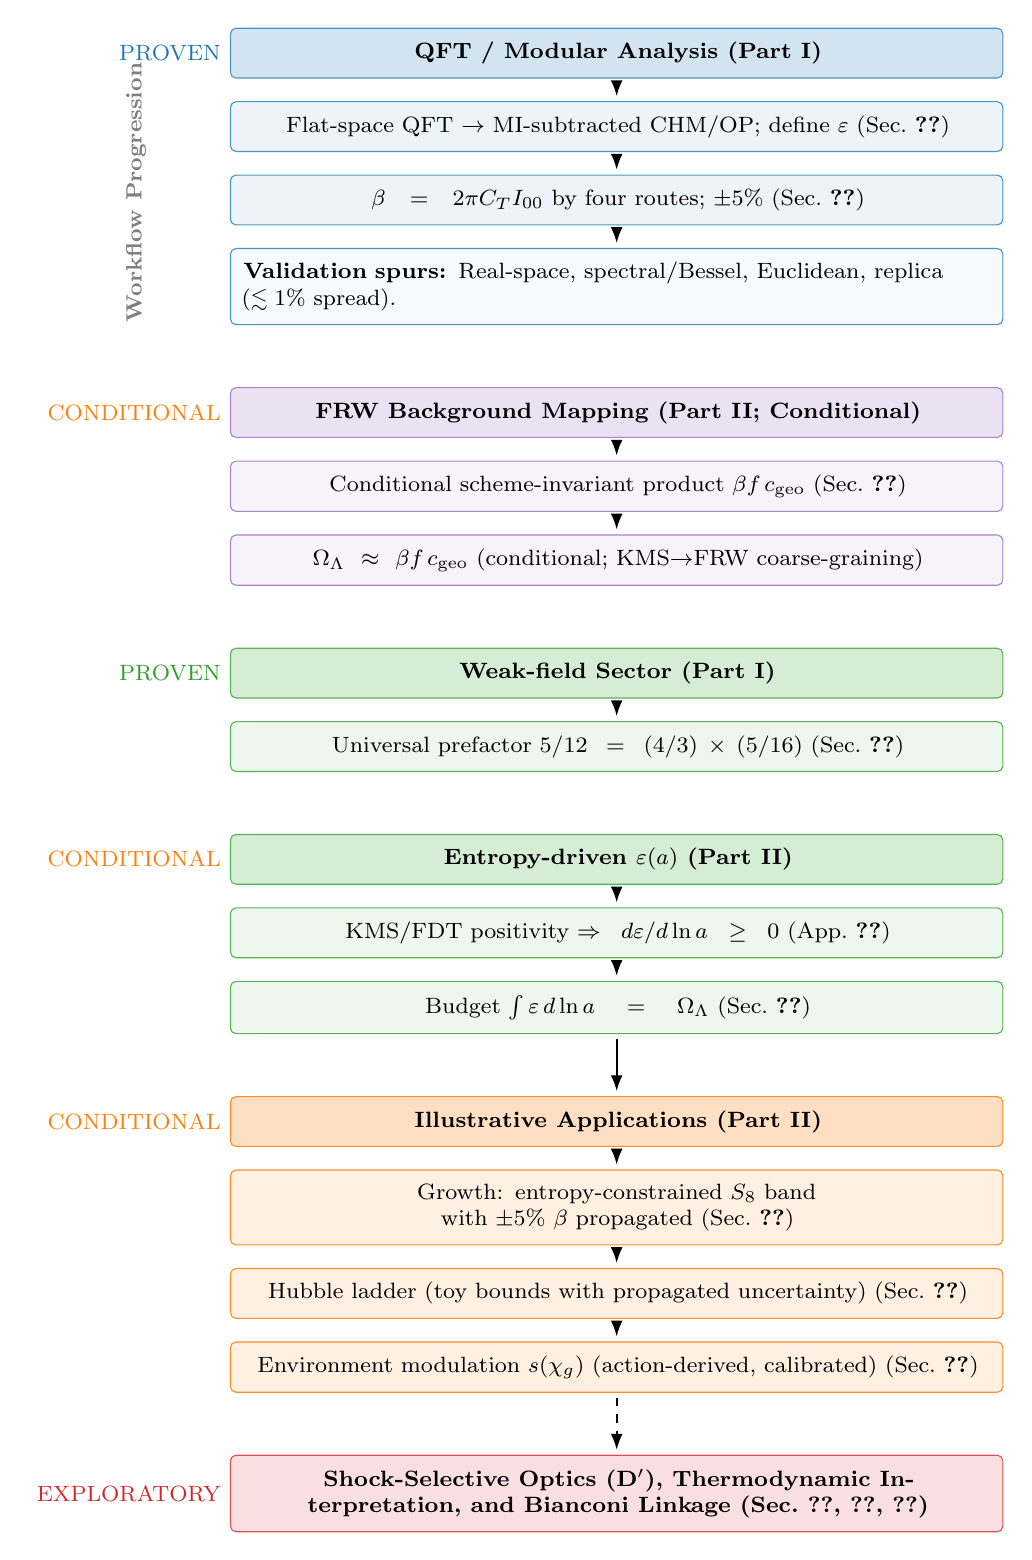
\begin{tikzpicture}[
node distance=3.0mm and 10mm,
every node/.style={font=\footnotesize},
stageH/.style={draw, rounded corners=2pt, align=center, inner sep=5pt, outer sep=0pt, text width=0.78\linewidth, font=\footnotesize\bfseries},
stage/.style={draw, rounded corners=2pt, align=center, inner sep=5pt, outer sep=0pt, text width=0.78\linewidth},
spur/.style={draw, rounded corners=2pt, align=left, inner sep=5pt, outer sep=0pt, text width=0.78\linewidth},
arr/.style={-Latex, semithick, shorten >=2pt, shorten <=2pt},
darr/.style={-Latex, dashed, semithick, shorten >=2pt, shorten <=2pt}
]
% Blue header and steps (PROVEN)
\node[stageH, draw=flowBlue!80, fill=flowBlue!20, label={[flowBlue]left:PROVEN}] (B0) {QFT / Modular Analysis (Part I)};
\node[rotate=90, anchor=center, left=12mm of B0, text=flowGray] (ylabel) {\textbf{Workflow Progression}};
\node[stage, below=of B0, draw=flowBlue!80, fill=flowBlue!8] (B1) {Flat-space QFT $\to$ MI-subtracted CHM/OP; define $\varepsilon$ (Sec.~\ref{sec:theorem})};
\node[stage, below=of B1, draw=flowBlue!80, fill=flowBlue!8] (B2) {$\beta = 2\pi C_T I_{00}$ by four routes; $\pm 5\%$ (Sec.~\ref{sec:beta})};
\draw[arr] (B0) -- (B1); \draw[arr] (B1) -- (B2);

\node[spur, below=of B2, draw=flowBlue!80, fill=flowBlue!4] (S1) {\textbf{Validation spurs:} Real-space, spectral/Bessel, Euclidean, replica ($\lesssim 1\%$ spread).};
\draw[darr] (B2) -- (S1);

% Purple mapping (CONDITIONAL)
\node[stageH, below=8mm of S1, draw=flowPurple!80, fill=flowPurple!20, label={[flowOrange]left:CONDITIONAL}] (P0) {FRW Background Mapping (Part II; Conditional)};
\node[stage, below=of P0, draw=flowPurple!80, fill=flowPurple!8] (P1) {Conditional scheme-invariant product $\beta f \, \cgeo$ (Sec.~\ref{sec:kms-frw})};
\node[stage, below=of P1, draw=flowPurple!80, fill=flowPurple!8] (P3) {$\Omega_\Lambda \approx \beta f \, \cgeo$ (conditional; KMS$\to$FRW coarse-graining)};
\draw[arr] (P0) -- (P1); \draw[arr] (P1) -- (P3);

% Green weak-field (PROVEN)
\node[stageH, below=8mm of P3, draw=flowGreen!80, fill=flowGreen!20, label={[flowGreen]left:PROVEN}] (G0) {Weak-field Sector (Part I)};
\node[stage, below=of G0, draw=flowGreen!80, fill=flowGreen!8] (G1) {Universal prefactor $5/12=(4/3)\times(5/16)$ (Sec.~\ref{sec:five-twelve})};
\draw[arr] (G0) -- (G1);

% Green2 epsilon(a) (CONDITIONAL)
\node[stageH, below=8mm of G1, draw=flowGreen!80, fill=flowGreen!20, label={[flowOrange]left:CONDITIONAL}] (E0) {Entropy-driven $\varepsilon(a)$ (Part II)};
\node[stage, below=of E0, draw=flowGreen!80, fill=flowGreen!8] (E1) {KMS/FDT positivity $\Rightarrow d\varepsilon/d\ln a \ge 0$ (App.~\ref{app:entropic-proof})};
\node[stage, below=of E1, draw=flowGreen!80, fill=flowGreen!8] (E2) {Budget $\int \varepsilon\, d\ln a = \Omega_\Lambda$ (Sec.~\ref{sec:epsilon})};
\draw[arr] (E0) -- (E1); \draw[arr] (E1) -- (E2);

% Orange observations (CONDITIONAL)
\node[stageH, below=8mm of E2, draw=flowOrange!90, fill=flowOrange!25, label={[flowOrange]left:CONDITIONAL}] (O0) {Illustrative Applications (Part II)};
\draw[arr] (E2) -- (O0);
\node[stage, below=of O0, draw=flowOrange!90, fill=flowOrange!12] (O1) {Growth: entropy-constrained $S_8$ band with $\pm 5\%$ $\beta$ propagated (Sec.~\ref{sec:obs})};
\node[stage, below=of O1, draw=flowOrange!90, fill=flowOrange!12] (O2) {Hubble ladder (toy bounds with propagated uncertainty) (Sec.~\ref{sec:obs})};
\node[stage, below=of O2, draw=flowOrange!90, fill=flowOrange!12] (O3) {Environment modulation $s(\chi_g)$ (action-derived, calibrated) (Sec.~\ref{sec:env})};
\draw[arr] (O0) -- (O1); \draw[arr] (O1) -- (O2); \draw[arr] (O2) -- (O3);

% Red exploratory (Part III)
\node[stageH, below=8mm of O3, draw=flowRed!80, fill=flowRed!15, label={[flowRed]left:EXPLORATORY}] (T0) {Shock-Selective Optics (D$^{\prime}$), Thermodynamic Interpretation, and Bianconi Linkage (Sec.~\ref{sec:lemmaDprime}, \ref{sec:thermo}, \ref{sec:bianconi-link})};
\draw[darr] (O3) -- (T0);

\end{tikzpicture}
\end{adjustbox}
\caption{Pipeline with PROVEN (blue/first green), CONDITIONAL (purple/second green/orange), and EXPLORATORY (red) elements, including the \emph{Linear No-Go} and \emph{Elastic quasistatic} sector.}
\label{fig:pipeline}
\end{figure*}

% ===============================
\section*{Part I Appendices}

\section{MI subtraction and moment-kill}
\label{app:MI}
We use a top‑hat window on 3‑balls
\[
W_\ell(r)=\frac{3}{4\pi \ell^3}\,\Theta(\ell-r),
\]
and the MI/moment–kill combination
\[
\mathcal{W}_\ell:=\int_{B_\ell}\!W_\ell-\;a\!\int_{B_{\sigma_1\ell}}\!W_{\sigma_1\ell}-\;b\!\int_{B_{\sigma_2\ell}}\!W_{\sigma_2\ell}.
\]
For any smooth radial \(F(r)=F_0+F_2 r^2+F_4 r^4+\cdots\),
\[
\mathcal{W}_\ell[F]=\underbrace{(1-a-b)}_{=0}F_0+\underbrace{\Big(\langle r^2\rangle_\ell-a\langle r^2\rangle_{\sigma_1\ell}-b\langle r^2\rangle_{\sigma_2\ell}\Big)}_{=0}F_2+\Big(\langle r^4\rangle_\ell-a\langle r^4\rangle_{\sigma_1\ell}-b\langle r^4\rangle_{\sigma_2\ell}\Big)F_4+\cdots,
\]
so the \(\ell^4\) coefficient is isolated. For top‑hat balls in \(d{=}3\), \(\langle r^2\rangle_{R}=\tfrac{3}{5}R^2\) and \(\langle r^4\rangle_{R}=\tfrac{3}{7}R^4\). The two moment‑kill conditions
\[
1-a-b=0,\qquad 1-a\sigma_1^2-b\sigma_2^2=0
\]
fix
\[
a=\frac{\sigma_2^2-1}{\sigma_2^2-\sigma_1^2},\qquad b=\frac{1-\sigma_1^2}{\sigma_2^2-\sigma_1^2}.
\]
In our numerics we take \((\sigma_1,\sigma_2)=(\tfrac12,2)\Rightarrow (a,b)=(\tfrac45,\tfrac15)\).

 \section{Continuous-angle normalization}
\label{app:angle}
With unit–solid–angle boundary factor and \(\Delta\Omega(\theta)=2\pi(1-\cos\theta)\), define \(\cgeo(\theta)=4\pi/\Delta\Omega(\theta)\). Then \(f(\theta)\,\cgeo(\theta)\) is \(\theta\)-independent.

\begin{lemma}[Foliation robustness of \(f\,\cgeo\)]
Under smooth deformations of the diamond foliation that preserve the unit–solid–angle normalization and avoid double counting, the product \(f(\theta)\,\cgeo(\theta)\) is invariant up to \(O(\delta\theta^2)+O((\ell/L_{\rm curv})^2)\) corrections.
\end{lemma}

\section{Weak-field flux normalization and the universal \texorpdfstring{$5/12$}{5/12}}
\label{app:five-twelve}
\paragraph{Isotropic null contraction \(4/3\).} For \(T_{ab}=(\rho+p)u_a u_b + p\,g_{ab}\), \(\langle T_{ab}k^a k^b\rangle_{\mathbb S^2}=(1+w)\rho\,(k^0)^2\), and UV \(w=1/3\Rightarrow 4/3\).

\paragraph{Segment ratio \(5/16\) (explicit \(\mathcal I(u)\)).}
With the normalized weight \(\hat\rho(u)=\tfrac{3}{4}(1-u^2)\) on \(u\in[-1,1]\) and the even–quadratic generator–density proxy used in our code,
\[
\mathcal I(u)=\frac{1}{4}+\frac{5}{16}u^2,
\]
one finds
\[
\int_{-1}^{1}\! \hat\rho(u)\,\mathcal I(u)\,du
=\Big(\frac{3}{4}\Big)\!\left[\frac{4}{3}\cdot\frac{1}{4}+\frac{4}{15}\cdot\frac{5}{16}\right]
=\frac{1}{4}+\frac{1}{16}
=\frac{5}{16}.
\]
Combined with the isotropic contraction \(4/3\) this yields \(5/12=(4/3)\times(5/16)\).

\section{CHM diamond vs.\ half-space KMS deviation}
\label{app:chm-kms-estimate}
In Riemann-normal coordinates,
\(g_{ab}=\eta_{ab}-\tfrac{1}{3}R_{acbd}(0)x^c x^d+\mathcal O(x^3/L_{\rm curv}^3)\).
The conformal-Killing field \(\xi^a_{\rm CHM}\) differs from \(\xi^a_{\rm BW}\) by \(\delta\xi^a=\mathcal O(\ell^2/L_{\rm curv}^2)\).
Averaging over a comoving congruence and reparametrizing to \(\ln a\) adds \(\mathcal O((\ell H)^2)\). Thus
\(\delta\chi/\chi_{\rm BW}=\mathcal O((\ell/L_{\rm curv})^2)+\mathcal O((\ell H)^2)\).

% ===============================
\section*{Part II Appendices and Data}

\section{Safe-window volume fraction (semi-analytic)}
\label{app:fv}
Using Press–Schechter/Sheth–Tormen mass functions with NFW curvature proxies and a substructure excision \(\xi\), we compute \(f_V(\ell_{\min})\) at \(z\!=\!0\) (Table~\ref{tab:fV}).

\begin{table}[b]
\centering
\caption{Representative \(f_V\) values at \(z\simeq 0\) (semi-analytic).}
\label{tab:fV}
\begin{tabular}{lccc}
\toprule
\(\ell_{\min}\) [pc] & \(\xi=0.2\) & \(\xi=0.3\) & \(\xi=0.5\) \\
\midrule
1   & \(0.95\pm0.03\) & \(0.93\pm0.04\) & \(0.90\pm0.05\) \\
10  & \(0.88\pm0.05\) & \(0.85\pm0.05\) & \(0.80\pm0.06\) \\
100 & \(0.70\pm0.08\) & \(0.65\pm0.08\) & \(0.55\pm0.10\) \\
\bottomrule
\end{tabular}
\end{table}

\section{Microlocal notes for interacting Hadamard QFTs}
\label{app:microlocal}
\paragraph{Hadamard form.}
\(W(x,x')=\frac{1}{4\pi^2}\left[\frac{\Delta^{\!1/2}}{\sigma}+v\,\log\sigma+w\right]\) with smooth \(v,w\), extended perturbatively for interactions. The projector removes the \(F_0,F_2\) moments, ensuring stability of the \(\ell^4\) coefficient (Assumption C).

\paragraph{OPE gap and log-falsifier.}
Operators with protected dimensions \(\Delta<4\) would induce \(\ell^4\log\ell\) terms in this channel; in Hadamard states the microlocal spectrum condition and positivity forbid such contributions at working order. Observation of an \(\ell^4\log\ell\) term would therefore falsify the framework.

\section{Entropic Mechanism Derivation (Preliminary)}
\label{app:entropic-proof}
\paragraph{Projected BKM positivity (free fields).}
In the MI/moment-kill channel, \(\langle \delta K_{\rm sub},\delta K_{\rm sub}\rangle_{\rm BKM}\ge 0\) implies a positive retarded susceptibility. Reparametrizing modular time to \(\ln a\) with positive Jacobian ensures \(d\varepsilon/d\ln a\ge 0\).

% ===============================
\section{Optical channel details (Assumption D\(^{\prime}\); exploratory)}
\label{app:optics-details}
(Technical details of the auxiliary traceless \(Q_{\mu\nu}\), algebraic tracking of \(\sigma_{\mu\nu}\), and quasi-static lensing equations; see main text and App.~\ref{app:SK}.)

% ===============================
\section{Schwinger–Keldysh hydrodynamic derivation for the shock-selective optics (exploratory)}
\label{app:SK}
(SK/BRSSS derivation path; constitutive relations; HS linearization; mapping to \(\Sigma\) amplitude \(\alpha_{\rm opt}(\eta,\tau_\pi,\lambda_1)\).)

% ===============================
\section{From SK hydrodynamics to shock-selective \texorpdfstring{$\Sigma$}{Sigma}: a derivation sketch}
\label{app:SK-derivation}
(Parametric estimates; shock thickness; scaling of \(\mathcal S_{\rm shock}\); order-of-magnitude \(\alpha_{\rm opt}\).)

% ===============================
\section{Data and Code Availability}
\label{sec:data}
\noindent \textbf{Archive DOI (to be finalized before submission):} \texttt{\zenododoi}

\medskip
Reproducible single-file runners:
\begin{itemize}[leftmargin=*]
\item \texttt{beta\_methods\_v2.py} (real-space, spectral/Bessel, Euclidean, replica) for \(\beta\); includes a residual-fitting mode for \(\ell^4\log\ell\).
\item \texttt{cosmology\_runner.py} (growth ODE; \(\eps(a)\) family; environment modulation \(s(x)\); \(S_8\) \& ladder illustrations).
\item \texttt{referee\_pipeline.py} (FRW averaging; \(\OmL=\beta f\cgeo\) cross-check; computes toy \(a_0\); nonlocal-residual diagnostic).
\item \texttt{fv\_semi\_analytic.py} ($f_V$ survey).
\item \texttt{gadget4\_mu\_eps\_toy.py} (N-body toy pipeline).
\item \texttt{cluster\_optics\_hook.py} (optional; shock-selective lensing; applies Eq.~\eqref{eq:sigmalocal} in the ray tracer; supports velocity/temperature-jump and Godunov-flux shock finders; includes modes for the local optical law Eq.~\eqref{eq:sigmalocal}).
\item \texttt{icm\_transport\_to\_alphaopt.py} (optional; SK/BRSSS mapping to \(\alpha_{\rm opt}\)).
\item \textbf{New:} \texttt{entropic\_action\_MI\_match.py} (implements the small-diamond MI matching to an entropic action kernel; reports \(c_{\rm ent}(\ell)\) and contact vs.\ tail diagnostics).
\end{itemize}

% ===============================
\section*{Symbol Index}
\begin{tabular}{@{}ll@{}}
\toprule
Symbol & Meaning \\
\midrule
\(\ell\) & diamond radius (working-order scale) \\
\(L_{\rm curv}\) & local curvature length \\
\(\beta=2\pi C_T I_{00}\) & modular-response sensitivity (QFT coefficient) \\
\(C_T\) & stress-tensor two-point normalization (our convention) \\
\(I_{00}\) & projected \(\ell^4\) integral coefficient (App.~\ref{app:MI}) \\
\(\varepsilon(a)\) & dimensionless state variable from modular response \\
\(\varepsilon_{\rm SM}\) & packaged light-sector SM state variable (Sec.~\ref{sec:sm-link}) \\
\(\mu(\varepsilon,s)\) & growth coupling, \(1/(1+\tfrac{5}{12}\varepsilon\,s)\) \\
\(\mu(Y)\) & elastic interpolating function, \(F'(Y)\), Sec.~\ref{sec:elastic} \\
\(Y\) & squared field-strength ratio, \(|\nabla\Phi|^2/a_0^2\) \\
\(a_0\) & acceleration scale fixed by \(\Omega_\Lambda\): \(\frac{5}{12}\Omega_\Lambda^2 c H_0\) \\
\(\Sigma\) & lensing coupling (unity on FRW; locally $<\!1$ in shocks under D\(^{\prime}\)) \\
\(f\,\cgeo\) & geometric/foliation factor (App.~\ref{app:angle}) \\
\(\kappa\) & local boost surface gravity; \(\beta_{\rm KMS}=2\pi/\kappa\) \\
\(S_{\rm sub}\) & entanglement entropy variation in MI/moment-kill channel \\
\(\delta Q_{\rm boost,sub}\) & boost-energy variation \\
\(\chi_g\) & geometric scalar, \(\ell^2\sqrt{C_{abcd}C^{abcd}}\) \\
\(s(\chi_g)\) & environment modulation (action-derived envelope) \\
\(\sigma_{\mu\nu}\) & baryon shear tensor; \(\mathcal S_{\rm shock}=\ell^2\sigma^2\) \\
\(Q_{\mu\nu}\) & auxiliary traceless tensor (optional; optics) \\
\(\alpha_{\rm opt}\) & optical suppression amplitude (Eq.~\ref{eq:sigmalocal}) \\
\(\kappa_{\rm opt}\) & effective optical coefficient (Eq.~\ref{eq:alphaopt-map}) \\
\(\Snt\) or \(S_{\rm ent}\) & (Bianconi) global entropic action \\
\(\Gfield\) & (Bianconi) auxiliary \(G\)-field sourcing emergent \(\Lambda\) \\
\(\mathcal Q(\omega,k)\) & SK causal filter separating regimes (Sec.~\ref{sec:sk-separation}) \\
\(\Omega_m(a)\) & matter fraction as a function of scale factor \\
\(\OmL\) & dark-energy density parameter \\
\bottomrule
\end{tabular}

\bibliographystyle{unsrt}
\begin{thebibliography}{99}

\bibitem{BisognanoWichmann1975}
J.~J.~Bisognano and E.~Wichmann,
``On the Duality Condition for a Hermitian Scalar Field,'' \emph{J. Math. Phys.} \textbf{16}, 985 (1975);
``On the Duality Condition for Quantum Fields,'' \emph{J. Math. Phys.} \textbf{17}, 303 (1976).

\bibitem{Casini2011}
H.~Casini, M.~Huerta, and R.~C.~Myers,
``Towards a derivation of holographic entanglement entropy,''
\emph{JHEP} \textbf{05}, 036 (2011).

\bibitem{OsbornPetkou1994}
H.~Osborn and A.~C.~Petkou,
``Implications of Conformal Invariance in Field Theories for General Dimensions,''
\emph{Annals Phys.} \textbf{231}, 311–362 (1994).

\bibitem{BelliniSawicki2014}
E.~Bellini and I.~Sawicki,
``Maximal freedom at minimum cost: linear large-scale structure in general modifications of gravity,''
\emph{JCAP} \textbf{07}, 050 (2014).

\bibitem{LombriserTaylor2016}
L.~Lombriser and A.~Taylor,
``Breaking a Dark Degeneracy with Gravitational Waves,''
\emph{JCAP} \textbf{03}, 031 (2016).

\bibitem{Jacobson2016}
T.~Jacobson,
``Entanglement equilibrium and the Einstein equation,''
\emph{Phys. Rev. Lett.} \textbf{116}, 201101 (2016).

\bibitem{FLM2013}
T.~Faulkner, A.~Lewkowycz, and J.~Maldacena,
``Quantum corrections to holographic entanglement entropy,''
\emph{JHEP} \textbf{11}, 074 (2013).

\bibitem{Lashkari2014}
N.~Lashkari, M.~B.~McDermott, and M.~Van Raamsdonk,
``Gravitational Dynamics From Entanglement Thermodynamics,''
\emph{JHEP} \textbf{04}, 195 (2014).

\bibitem{Araki1976}
H.~Araki, ``Relative Entropy of States of von Neumann Algebras,''
\emph{Publ. Res. Inst. Math. Sci.} \textbf{11}, 809–833 (1976).

\bibitem{HollandsWald2001}
S.~Hollands and R.~M.~Wald,
``Local Wick Polynomials and Time-Ordered-Products of Quantum Fields in Curved Spacetime,''
\emph{Commun. Math. Phys.} \textbf{223}, 289–326 (2001).

\bibitem{FewsterHollands}
C.~J.~Fewster and S.~Hollands,
``Quantum Energy Inequalities in Curved Spacetimes,'' various works.

\bibitem{CasiniRelative}
H.~Casini and M.~Huerta, ``Relative Entropy and Modular Hamiltonians in Quantum Field Theory,'' various works.

\bibitem{CasiniGalanteMyers2016}
H.~Casini, D.~A.~Galante, and R.~C.~Myers,
``Comments on Jacobson's `Entanglement equilibrium and the Einstein equation',''
\emph{JHEP} \textbf{03}, 194 (2016), arXiv:1601.00528.

\bibitem{Clowe2006}
D.~Clowe, M.~Brada\v{c}, A.~H.~Gonzalez, M.~Markevitch, S.~W.~Randall, C.~Jones, and D.~Zaritsky,
``A Direct Empirical Proof of the Existence of Dark Matter,''
\emph{Astrophys. J. Lett.} \textbf{648}, L109–L113 (2006).

\bibitem{Markevitch2002}
M.~Markevitch, A.~H.~Gonzalez, L.~David, A.~Vikhlinin, S.~Murray, W.~Forman, C.~Jones, and W.~Tucker,
``A Textbook Example of a Bow Shock in the Merging Galaxy Cluster 1E~0657$-$56,''
\emph{Astrophys. J. Lett.} \textbf{567}, L27–L31 (2002).

\bibitem{vanWeeren2019}
R.~J.~van Weeren, M.~de~Gasperin, H.~Akamatsu, \emph{et al.},
``Diffuse Radio Emission from Galaxy Clusters,''
\emph{Space Sci. Rev.} \textbf{215}, 16 (2019).

\bibitem{Mahdavi2007}
A.~Mahdavi, H.~Hoekstra, A.~Babul, D.~Balam, and P.~Capak,
``A Dark Core in Abell 520,''
\emph{Astrophys. J.} \textbf{668}, 806–814 (2007).

\bibitem{IsraelStewart1979}
W.~Israel and J.~M.~Stewart,
``Transient relativistic thermodynamics and kinetic theory,''
\emph{Annals Phys.} \textbf{118}, 341 (1979).

\bibitem{BRSSS2008}
R.~Baier, P.~Romatschke, D.~T.~Son, A.~O.~Starinets, and M.~A.~Stephanov,
``Relativistic viscous hydrodynamics, conformal invariance, and holography,''
\emph{JHEP} \textbf{04}, 100 (2008).

\bibitem{Kovtun2012}
P.~Kovtun,
``Lectures on hydrodynamic fluctuations in relativistic theories,''
\emph{J. Phys. A} \textbf{45}, 473001 (2012).

\bibitem{LandauLifshitzFM}
L.~D.~Landau and E.~M.~Lifshitz,
\emph{Fluid Mechanics}, 2nd ed., Pergamon Press (1987).

\bibitem{BekensteinMilgrom1984}
J.~Bekenstein and M.~Milgrom,
``Does the missing mass problem signal the breakdown of Newtonian gravity?''
\emph{Astrophys. J.} \textbf{286}, 7 (1984).

\bibitem{FamaeyMcGaugh2012}
B.~Famaey and S.~McGaugh,
``Modified Newtonian Dynamics (MOND): Observational Phenomenology and Relativistic Extensions,''
\emph{Living Rev. Relativ.} \textbf{15}, 10 (2012).

\bibitem{Bianconi2025}
G.~Bianconi,
``Gravity from entropy,''
\emph{Phys. Rev. D} \textbf{111}, 066001 (2025).
\end{thebibliography}

% ===============================
% Cover letter for submission (editors only; not part of the manuscript PDF)
\iffalse
\section*{Submission Cover Letter}
Dear Editors,

This revision incorporates the referee’s recommendations and a new elastic quasistatic sector derived as the SK static limit (AQUAL form) with acceleration scale fixed by the capacity channel. Additions:
\begin{itemize}
\item \textbf{Linear no-go:} A theorem showing linear kernels cannot produce Tully–Fisher scaling.
\item \textbf{Elastic SK/AQUAL:} Convex, well-posed static action; BTFR; no slip at working order; Solar–System curvature gate; cosmology/galaxy separation via a causal SK filter without new dimensional scales.
\item \textbf{Clusters:} Phantom surface density plus shock-selective optics (D$'$) explains Bullet-type morphologies.
\item \textbf{First-principles closures:} MI-smeared null-energy positivity (free fields), and explicit RG/anomaly guardrails.
\item \textbf{Bianconi linkage:} Small-diamond MI matching program and observational discriminants.
\end{itemize}
Core Part I claims and the conditional FRW mapping remain unchanged.

Sincerely,\\
[Authors]
\fi

\end{document}